\documentclass[tikz,border=5pt]{standalone}
\usepackage{tikz}
\usetikzlibrary{arrows.meta,positioning}
\definecolor{nebula}{HTML}{6366F1}
\definecolor{spark}{HTML}{14B8A6}
\definecolor{ink}{HTML}{334155}
\begin{document}
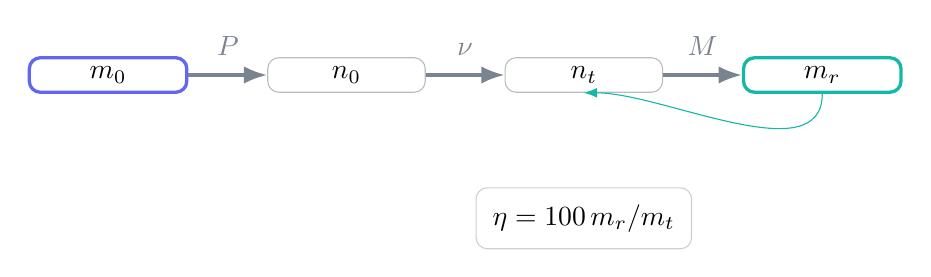
\begin{tikzpicture}[font=\sffamily,>=Latex,node distance=1cm]
  \node[draw=nebula,very thick,rounded corners=4pt,minimum width=2cm] (m) {$m_0$};
  \node[draw=ink!35,rounded corners=4pt,right=of m,minimum width=2cm] (n) {$n_0$};
  \node[draw=ink!35,rounded corners=4pt,right=of n,minimum width=2cm] (nt) {$n_t$};
  \node[draw=spark,very thick,rounded corners=4pt,right=of nt,minimum width=2cm] (mr) {$m_r$};
  \draw[->,very thick,ink!65] (m)--(n) node[midway,above=3pt] {$P$};
  \draw[->,very thick,ink!65] (n)--(nt) node[midway,above=3pt] {$\nu$};
  \draw[->,very thick,ink!65] (nt)--(mr) node[midway,above=3pt] {$M$};
  \node[below=1.2cm of nt,draw=ink!25,rounded corners=4pt,fill=white,inner sep=6pt]
    {$\eta=100\,m_r/m_t$};
  \draw[->,spark] (mr.south) .. controls +(0,-1) and +(1,0) .. (nt.south);
\end{tikzpicture}
\end{document}
